\documentclass[a4paper,10pt,twoside]{article}
%%%%%%%%%%% Packages %%%%%%%%%%
\usepackage[margin=1in]{geometry}
\usepackage{amsmath, amssymb,mathtools}
\usepackage{fancyhdr}
\usepackage{sectsty}
\usepackage{graphicx,wrapfig}
\usepackage{enumitem}
\usepackage{float}
\usepackage{braket}
\usepackage{bbm}
\usepackage{tikz,calc}

%%%%%%%%%%% Macros %%%%%%%%%%
\def \note#1 {\vspace{-1em}\paragraph{\bfseries #1}}
\def \dd {{\rm d}}
\def \id {{\mathbbm{1}}}
\def \order {\mathcal{O}}
\def\bquad{\mkern-18mu}
\DeclareMathOperator{\trace}{tr}
\DeclareMathOperator{\spanset}{span}

%%%%%%%%%%% Tikz Definitions %%%%%%%%%%
\usetikzlibrary{shapes, arrows,positioning,fit}
\tikzstyle{plain} = [draw,thick,circle,inner sep=0,minimum size=0.5cm,font=\footnotesize]
\tikzstyle{mps} = [draw,thick,rectangle,rounded corners=.1cm,inner sep=0,minimum size=0.5cm]
\tikzstyle{mpo} = [draw,thick,circle,inner sep=0,minimum size=0.5cm]
\tikzstyle{index} = [-,thick,font=\footnotesize]
\tikzstyle{virtual} = [-,thick,dotted,font=\footnotesize]
\tikzstyle{site} = [draw,solid,circle,minimum size=2pt,inner sep=0pt,outer sep=0pt,fill=black]

\def \tu {0.25cm}

%%%%%%%%%%% Formatting %%%%%%%%%%
\pagestyle{fancy}
\renewcommand{\footrulewidth}{0.5pt}

\fancyhf{}
\lhead{08/06/2017}
\chead{Quantum Information Methods in Many-Body Physics}
\rhead{PH2269}
\lfoot{Giacomo Giudice~~~~giacomo.giudice@mpq.mpg.de}
\rfoot{Page \thepage}

\allsectionsfont{\normalfont\sffamily}

%%%%%%%%%%% Here Begins Document %%%%%%%%%%
\begin{document}
\title{\vspace{-1cm}\sffamily Homework 6\vspace{-1cm}}
\author{}
\date{}
\maketitle
\thispagestyle{fancy}

\begin{section}{Area Law for the Toric Code}
Consider an area $A$ of the toric code ground state $\ket{\Psi}$.
Notice that all the loop configurations intersect $\partial A$ an even number of times. 
Why is that?
We shall call the configurations of highlighted links crossing $\partial A$ a \emph{boundary pattern}.
Show that, for a given $A$,  the number of loop configurations in the interior of $A$ is independent of the boundary pattern.

We can write a Schmidt decomposition $\ket{\Psi} = \sum_i \lambda_i \ket{\alpha_i} \ket{\beta_i}$, with states $\ket{\alpha_i}$ belonging to $A$ and $\ket{\beta_i}$ belonging to $\bar{A}$.
Prove that, in this case,
\[
   \ket{\Psi} = \frac{1}{\sqrt{\mathcal{N}_B}}\sum_{i=1}^{\mathcal{N}_B} \ket{\alpha_i} \ket{\beta_i},
\]
where $\mathcal{N}_B$ is the number of boundary patterns.
How much is $\mathcal{N}_B$?
Conclude by showing that the entanglement is $S_A = |\partial A| - 1$.
What is the topological correction to the area law for the toric code?

\note{Hint} Compute many loops can you construct on a generic area of the lattice by repeatedly applying the plaquette operator.
\end{section}

\begin{section}{The Toric Code as a PEPS}
Recall the construction of the toric code ground state using the tensor below
\[
  A^{i_1,i_2,i_3,i_4}_{\alpha,\beta,\gamma,\delta}
  = 
  {
    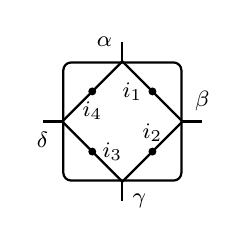
\begin{tikzpicture}[baseline=0]
      \node[mps,minimum size=6*\tu] (t) {};
      \draw[index] (t.north) -- +(0,\tu) node[left]{$\alpha$};
      \draw[index] (t.east) -- +(\tu,0) node[above]{$\beta$};
      \draw[index] (t.south) -- +(0,-\tu) node[right]{$\gamma$};
      \draw[index] (t.west) -- +(-\tu,0) node[below]{$\delta$};
      \draw[index] (t.north) -- (t.east) node[site,midway]{} node[midway,left]{$i_1$};
      \draw[index] (t.east) -- (t.south) node[site,midway]{} node[midway,above]{$i_2$};
      \draw[index] (t.south) -- (t.west) node[site,midway]{} node[midway,right]{$i_3$};
      \draw[index] (t.west) -- (t.north) node[site,midway]{} node[midway,below]{$i_4$};
    \end{tikzpicture} 
  }
  = 
  \begin{cases}
    \alpha=i_4 \oplus i_1\\
    \beta=i_1 \oplus i_2\\
    \gamma=i_2 \oplus i_3\\
    \delta=i_3 \oplus i_4\\
  \end{cases} ,
\]
where $\oplus$ is the logical XOR operation, i.e. addition modulo 2.
\begin{enumerate}[label=(\alph*)]
\item List all the configurations that give rise to a non-zero entry of $A$.
Do this by graphically highlighting the physical and virtual links associated to the index 1. 
You should obtain 16 distinct configurations.
\item What is the action of $X$ from a physical leg to the virtual legs? 
What about a pair of $X$s or $Z$s on different physical legs?
\item Check that the tensor $A$ is $\mathrm{Z}_2$-invariant on the virtual level.
\item Show the symmetries of the toric code $A_v \ket{\Psi} = \ket{\Psi}$ and $B_p \ket{\Psi} = \ket{\Psi}$ using the tensor.
\item How do the string operators $W_l^{(e)}$ and $W_{l^*}^{(m)}$ (see previous homework) act on the tensors?
What are the endpoint tensors and how do they transform under the $\mathrm{Z}_2$ symmetry?
What about closed loops?
\item Prove that the contraction of all these different tensors gives rise to all loop configurations, with the same weight.
\end{enumerate}
\end{section}

\newpage

\begin{section}{The Toric Code on the Honeycomb Lattice*}
\begin{figure}[h]
  \centerline{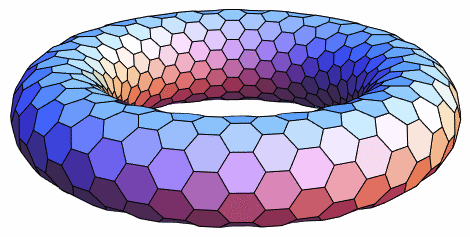
\includegraphics[width=0.3\textwidth]{img/torus.png}}
\end{figure}
Consider a honeycomb lattice on a torus, with a qubit on each edge.
As for the square lattice, we define a toric code Hamiltonian for this lattice.
How many degenerate ground states do you expect?
We will now derive the physics of this model, in a similar fashion to the square lattice case.
\begin{enumerate}[label=(\alph*)]
\item Write down the vertex and plaquette operators, in terms of the Pauli matrices, using the same convention used during the lectures.
 Denote the ($-1$)-eigenstate of $Z$ by a highlighted edge.
What are all the 1-eigenstates of the vertex term?
\item Formulate the ground space as a sum over loop configurations. 
What additional properties do these loop configurations have, compared to the square lattice case?
\item Construct a tensor network associated to this ground state. 
Construct a copy of each site by adding an ancillary state $\ket{0}$ to each edge and applying a CNOT gate on the pair.
We can then construct a tensor $A^{i_1,i_2,i_3}_{\alpha,\beta,\gamma}$ for three sites around each vertex.
Which configurations give rise to a non-zero entry to the tensor?
\item Check that this tensor has a purely virtual $\mathrm{Z}_2$ symmetry.
\item So far we have been a bit generic on the boundary conditions.
Consider the two polygons below, where each boundary is glued to its matching one. 
What surfaces do these constructions generate? 
Are they topologically equivalent?
\begin{figure}[h]
  \centerline{
    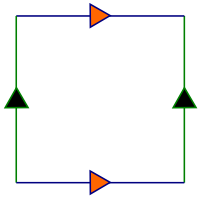
\includegraphics[width=0.12\textwidth]{img/fundamental_square.png}
    \hspace{4em}
    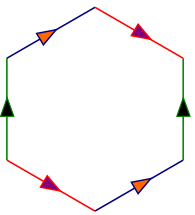
\includegraphics[width=0.12\textwidth]{img/fundamental_hex.png}
  }
\end{figure}
\item Can we cover these surfaces with a honeycomb lattice? 
If so, what is the degeneracy of the ground state of the toric code on each surface?
\end{enumerate}
\end{section}
\end{document}
%%%%%%%%%%% Here Ends Document %%%%%%%%%%
